%===================================== CHAP 3 =================================

\chapter{Previous Work}

The work presented in this thesis extends the Cellular Automata Research
Platform (CARP), an FPGA-based system implemented specifically to support and
accelerate research into growth and evolution of developmental systems based on
cellular automata. The original implementation was done by Djupdal in 2003. Over
the years, the system has been extended as well as optimized to run on newer
hardware through a series of master theses. The following sections provide an
overview of the evolution of the system.

\figurename~\ref{fig:overview-general} shows the original overall design of the
system, indicating how the host program is responsible for evolving genotypes,
while developing genotypes into phenotypes and simulating their behaviour in the
CA is implemented on the FPGA.

\begin{figure}[ht]
  \centering
  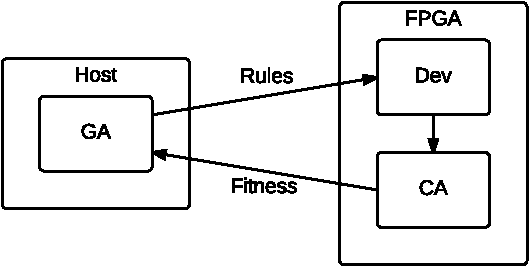
\includegraphics[width=0.6\linewidth]{fig/overview-general}
  \caption[General system design]{General system design. Figure taken from \cite{Lundal2015a}.\label{fig:overview-general} }
\end{figure}

%\section{Haddow \& Tufte}
%
%Possible section outlining the SBlock idea?

\section{Djupdal}

The original design of the CARP system was made by Djupdal in 2003
\cite{Djupdal2003}, to support further research into elvolvable hardware based
on the SBlock-architecture proposed by Tufte and Haddow \cite{Haddow2000a}. The
system was implemented on a NallaTech BenERA FPGA-board communicating over
\acrfull{pci} with a CompactPCI host-computer.

\figurename~\ref{fig:overview-djupdal} shows the overall architecture of the
resulting hardware platform. It consists of the SBlock Matrix (SBM), Block RAM
(BRAM) for storing the state and type of each cell, a development unit, control
logic, and a \acrshort{pci} communication unit.

\begin{figure}[!ht]
    \centering
    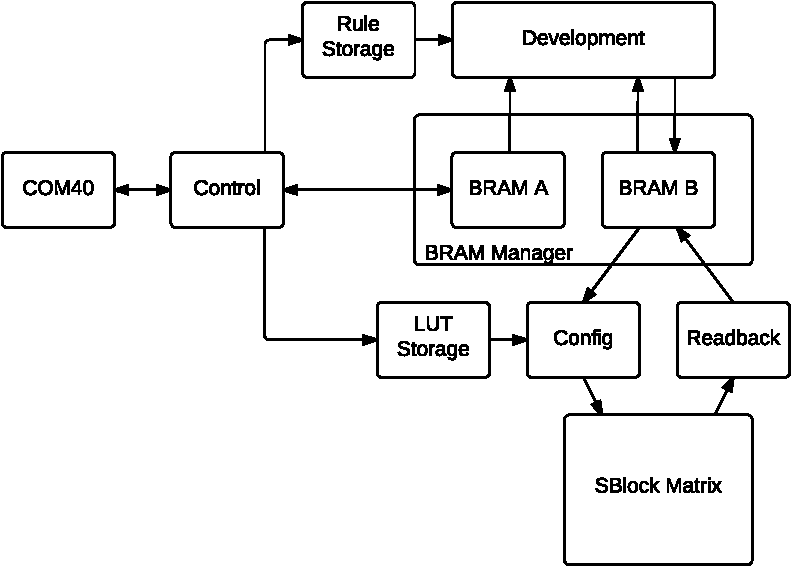
\includegraphics[width=0.8\linewidth]{fig/overview-djupdal}
    \caption[Djupdal's hardware design]{
        High-level block diagram of the hardware platform as implemented by
        Djupdal. Figure taken from \cite{Lundal2015a}.
    }
    \label{fig:overview-djupdal}
\end{figure}

A host computer, running a genetic algorithm exploring the space of possible
development rules, controls the system. Each genotype is transferred to the
system and developed into its phenotype before the SBM is stepped some number of
times. New states and types can then be transferred back to the host to
calculate a fitness score.

A genotype consists of a set of initial cell states and types, development rules
and LUTs corresponding to the cell types possible. Upon initializing the system
with a new genotype, states and types are written to BRAM A, while development
rules and LUTs have their own separate BRAMs. During development, cells are read
from BRAM A, tested against development rules and written back to BRAM B, now possibly
changed as a result of ``hitting'' a rule. The development unit tests 8 rules on
2 cells each cycle in raster order. This means that for sets of rules larger
than 8, several sweeps over the cells is necessary. For these additional sweeps,
cells are read from BRAM B so as not to overwrite the result of a rule hit in a
previous sweep if no rules hit in the later ones. The two BRAMs can be swapped
logically, avoiding having to transfer between the two in order to start a new
development step.

Based on the cell types stored in BRAM A, the SBM can be configured. Each cell
type corresponds to a LUT stored in the LUT storage BRAM, with which the SBlocks
corresponding to cells of that type is configured. State steps can then be
performed either one at a time, writing each new set of states back to BRAM B,
or in batches, writing only the final set of states back.

\section{Aamodt}

In Djupdals design it was necessary to transfer cell states to the host to
calculate fitness. To avoid this bottleneck, Aamodt extended the system with an
on-board fitness module in 2005 \cite{Aamodt2005}. Additionally, to gain further
insight into the development process, he added logging-modules for the
development unit.

\figurename~\ref{fig:overview-aamodt} shows the overall system as implemented by
Aamodt. The modules added are as follows; a Run-Step Function (RSF) that
calculates the number of live cells, a BRAM module to buffer these numbers, a
fitness function and the two logging modules from the development unit.

\begin{figure}[!ht]
    \centering
    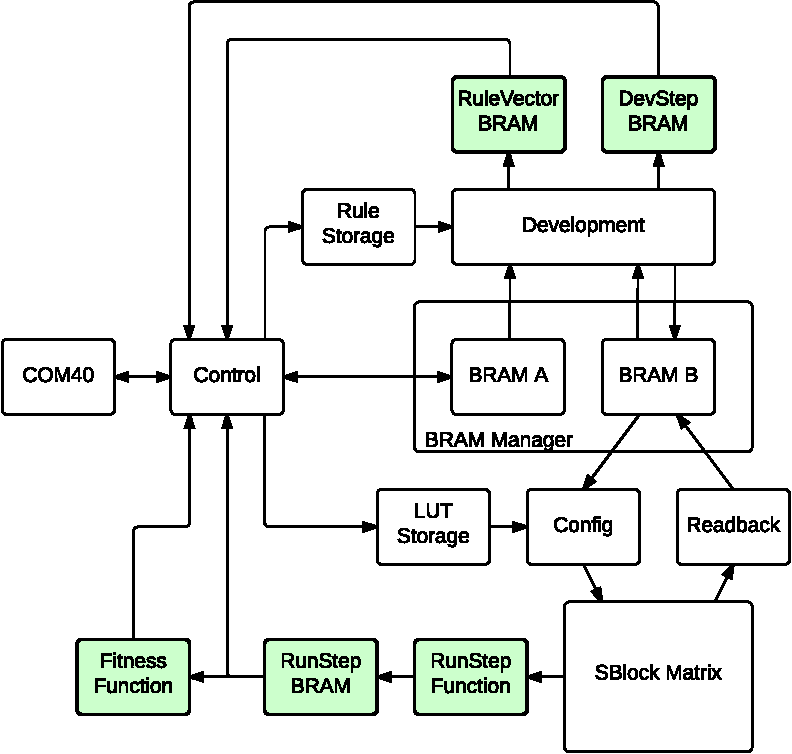
\includegraphics[width=0.8\linewidth]{fig/overview-aamodt}
    \caption[Aamodt's hardware design]{
        High-level block diagram of the hardware platform after Aamodt's work.
        Additions are highlighted in green. Figure taken from \cite{Lundal2015a}. 
    }
    \label{fig:overview-aamodt}
\end{figure}

The two BRAMs added to the development module logs information regarding the
development process. The Development Step BRAM stores wich rules were triggered
for all cells during the most recent development step, while the Rule Vector
BRAM stores which rules were triggered overall for the last 256 development
steps. The RSF is a large adder tree, calculating the total number of live cells
in the SBlock matrix after each state step. These totals are buffered in the
RunStep BRAM before being processed by the fitness function.

\section{Støvneng}

In 2014, the system was further extended and optimized by Støvneng
\cite{Stovneng2014}, in expectation of new FPGAs aquired by NTNU. In addition to
rewriting existing modules to better utilize the resources available on the new
chips, he also modified the SBlock matrix to allow for 3D CAs and implemented an
on-chip Discrete Fourier Transform (DFT) for processing the cell count from the
RSF-module into the frequency domain.

\begin{figure}[!ht]
    \centering
    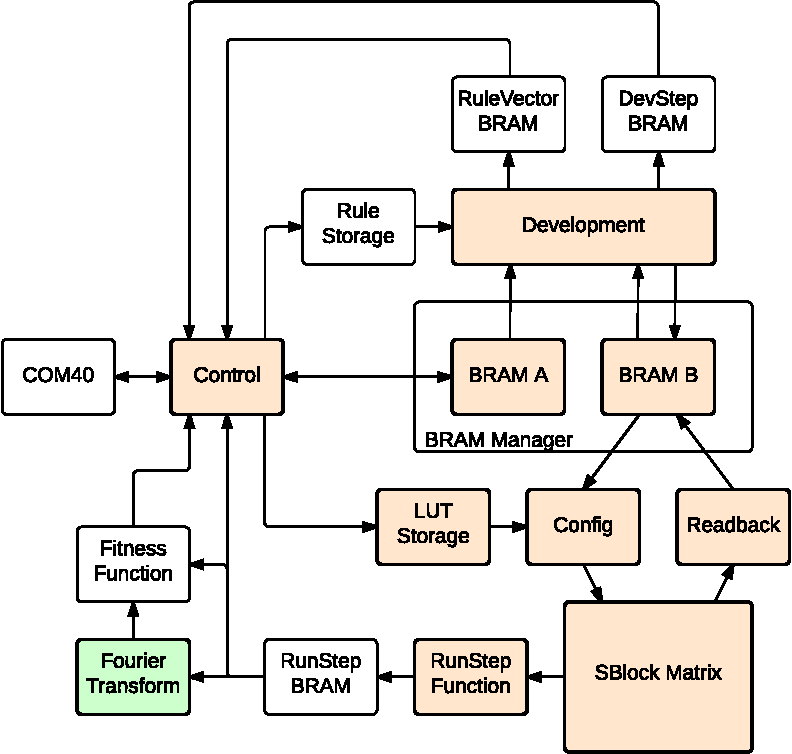
\includegraphics[width=0.8\linewidth]{fig/overview-stovneng}
    \caption[Støvneng's hardware design]{
        High-level block diagram of the hardware platform after Støvneng's work.
        Additions are highlighted in green, and optimizations and 3D modifications in orange.
        Figure taken from \cite{Lundal2015a}.
    }
    \label{fig:overview-stovneng}
\end{figure}

\figurename~\ref{fig:overview-stovneng} shows how the DFT module is added to the
overall design, as well as which modules have been optimized and rewritten to
support 3D CAs. Overall, the optimizations made to the system yielded a 4x
speedup for most operations. The design as a whole was also made more
parameterized and portable by removing many hard coded constants and rewriting
modules relying on features specific to the old FPGA.

As the new hardware did not arrive in time, Støvneng was unable to test his
changes on the actual FPGA, but the design in its entirety was verified through
simulation.

\section{Lundal}

After Støvneng finished his work, it became clear that the new hardware would be
delayed yet again. To allow for further development and testing of the platform
on actual hardware, a development board with a similar FPGA as the one in the
anticipated new hardware was ordered. As this newer line of FPGAs has removed
support for PCI in favor of PCIe, both the communication module on the hardware
platform and the software side driver had to be updated. While testing the new
communication module, several issues with the current implementation were uncovered,
such as commands not functioning according to specification and extensive use of
outdated FPGA features. This led to the decision of rewriting the platform from
scratch, a job undertaken by Lundal in 2015 \cite{Lundal2015a}.


\begin{figure}[ht]
  \centering
  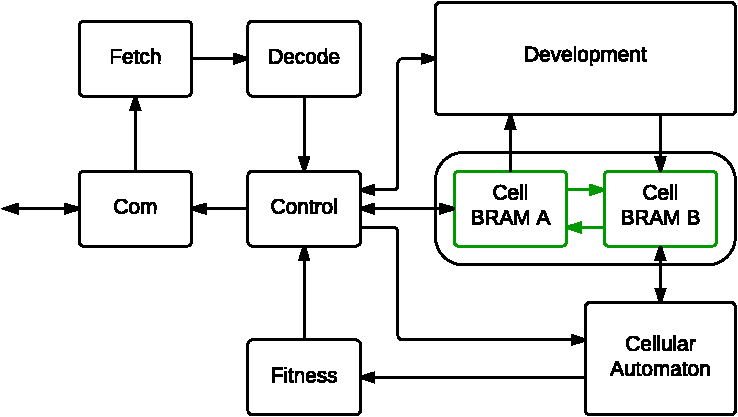
\includegraphics[width=0.8\linewidth]{fig/lundal-implementation-simple}
  \caption{
    Overview of the reorganized hardware platform as implemented by Lundal.
    Figure taken from \cite{Lundal2015a}. \label{fig:lundal-implementation-simple}
  }
\end{figure}

Through his work, Lundal focused on making the hardware platform more modular,
easier to configure and coherently structured. All dependencies on specific
hardware features have been removed in favor of letting the synthesizer infer
based on which resources are available on the targeted chipset. Support for both
2D and 3D SBMs was implemented by Aamodt as two separate designs. Lundal unified
this into one design, utilizing the fact that all 2D CAs can be implemented as
one-high 3D CAs. The software API was also made more complete and user-friendly,
by implementing abstractions that allow the end user to focus more on the code
related to the experiment being performed and less on the technicalities
necessary to operate the hardware platform.

Since Djupdals original design, the development module has remained largely
unchanged, implementing a developmental model based on research by Haddow and
Tufte \cite{Tufte2005a}. In this model two types of developmental rules are
considered; growth-rules indicating how an organism develops spatially, and
change rules describing how existing cells can change their type. Both rule
types consist of a condition and a result. Conditions take into account the
types of the cells in the von Neumann neighborhood around the target cell and
the type of the target cell itself. The result of a growth rule is the direction
in which the target cell should grow. For a change rule, the result is the new
type of the target cell. Change rules can only affect cells that have already
been grown into and growth rules can only grow into cells that are empty.

Lundal implemented a simpler development module based on Tufte and Nicheles
research \cite{Nichele2013}. Here, all rules are effectively change rules and all
rules are evaluated for all cells. The functionality of growth rules in the old
design can still be implemented within this scheme. Where the differentiation of
growth and change in the old design is closer to the type of cell development
that happens in biological systems, the new system is more applicable to generic
dynamical systems.

Lundal verified the reimplemented CARP platform both through simulation and
end-to-end integration tests with the synthesized design . 

\cleardoublepage

%%% Local Variables:
%%% mode: latex
%%% TeX-master: "../thesis"
%%% End:
